\documentclass[t]{beamer}

\usetheme{Frankfurt}
%\usecolortheme{beaver}
\usefonttheme{professionalfonts}
% Insert the frame number at the bottom line
\expandafter\def\expandafter\insertshorttitle\expandafter{%
  \insertshorttitle\hfill\insertframenumber\,/\,\inserttotalframenumber}
% Remove the navigation symbols (one of the two options)
%\usenavigationsymbolstemplate{}
\setbeamertemplate{navigation symbols}{}

\usepackage{graphicx,color,dashbox,amsmath}
\usepackage{hyperref}% embedding hyperlinks [must be loaded after dropping]
\usepackage{amsmath}
\usepackage{amsthm,amssymb,amsfonts,latexsym,mathrsfs,wasysym}
\usepackage{pifont}
\usepackage{marvosym}
\usepackage{subfigure}
\usepackage{epstopdf}
\usepackage{soul,color}
\usepackage{threeparttable}% tables with footnotes
\usepackage{dcolumn}% decimal-aligned tabular math columns
\usepackage{float}
\usepackage{algorithm}
\usepackage[noend]{algpseudocode}
%\usepackage{subfig}

%\usepackage[style=ieee,backend=bibtex,citestyle=ieee]{biblatex}
%\usepackage[multiple]{footmisc}
%\addbibresource{bibliography.bib}
%\usepackage{colortbl}

\usepackage{tikz}
\usetikzlibrary{calc}
\usetikzlibrary{shapes.geometric}
\usetikzlibrary{arrows.meta}

%\usepackage{enumitem}
%\newlist{arrowlist}{itemize}{1}
%\setlist[arrowlist]{label=$\Rightarrow$}

\newcolumntype{d}{D{.}{.}{-1}}
\graphicspath{{Figures/}}

\logo{
\includegraphics[width=3em]{lapid-logo-45}}
\renewcommand{\baselinestretch}{1.2}

% commands and colors
\newcommand{\rR}{\mathbb{R}}
\newcommand{\rsqr}{\mathbb{R}^2}
\newcommand{\rthrd}{\mathbb{R}^3}
\newcommand{\eqsn}[1]{\begin{equation}#1\end{equation}}
\newcommand{\br}{$\\ $}

\newcommand{\bmat}[1]{\begin{bmatrix}#1\end{bmatrix}}
\newcommand{\mat}[1]{\begin{matrix}#1\end{matrix}}
\newcommand{\vmat}[1]{\begin{vmatrix}#1\end{vmatrix}}

\newcommand{\con}{c\left(t\right)}
\newcommand{\conp}[1]{c_{#1}\left(t\right)}
\newcommand{\concov}{\mathtt{C}\left(\con\right)}
\newcommand{\concovp}[1]{\mathtt{C}\left(\conp{#1}\right)}
\newcommand{\conset}{\mathtt{G}}

\newcommand{\sigp}{\sigma\left(p\right)}
\newcommand{\sigpp}[2]{\sigma_{#1 #2}\left(p \right)}
\newcommand{\pb}{\bar{p}}

\newcommand{\norm}[1]{\lVert #1 \rVert}

\makeatletter
\newcommand{\mathleft}{\@fleqntrue\@mathmargin0pt}
\newcommand{\mathcenter}{\@fleqnfalse}
\makeatother


% Gilad New Commands
\newcommand{\sgn}[1]{\operatorname{sgn}\left(#1\right)}
\newcommand{\sat}[1]{\operatorname{sat}\left(#1\right)}
%\newcommand{\rrule}[1]{\rule[#1]{0pt}{0pt}}

%beamer@blendedblue
\definecolor{mgreen}{RGB}{40,160,40}
\definecolor{natigreen}{RGB}{50,205,50}
\definecolor{natiblue}{RGB}{0,191,255}
\definecolor{mg}{rgb}{0,0.4,0}%
\definecolor{mypink2}{RGB}{219, 48, 122}

\newtheorem*{Proposition}{Proposition}
\newtheorem*{keylemma}{Key Lemma}
\newtheorem*{Remark}{Remark}
\newtheorem*{question}{Question}
\newtheorem*{Task}{Task}
\newtheorem*{cor}{Corollary}
\newtheorem*{thm}{Theorem}

%%%%%%%%%%%%%%%%%%%%%%%%%%

\title{A Projected Lloyd’s Algorithm for Coverage Control Problems}

\author[Palti]
{Yoav Palti}

\institute[]
{Faculty of Aerospace Engineering, Technion - Israel Institude Of Technology}

\date[MSc Seminar]
{M.Sc. Seminar \\
Supervisor: Associate Professor Daniel Zelazo \\[1ex]
\footnotesize\em December 10, 2018}

\AtBeginSection[]
{
  \begin{frame}
    \frametitle{Table of Contents}
    \tableofcontents[currentsection]
  \end{frame}
}

\setbeamertemplate{blocks}[default]%[rounded][shadow=true]

%%%%%%%%%%%%%%%%%%%%%%%%%%
\begin{document}
\begingroup
% For the first slide only, remove all the text from the header/footer lines
\renewcommand*\insertshorttitle{}
\renewcommand*\insertshortauthor{}
\renewcommand*\insertshortinstitute{}
\renewcommand*\dohead{\rule{0em}{1.45em}}
\begin{frame}[label=sl1]
  \titlepage
\end{frame}
\endgroup

\begin{frame}
\frametitle{Table of Contents}
\tableofcontents
\end{frame}

%%%%%%%%%%%%%%%%%%%%%%%%%%%%%%%%%%%%%%%%%%
%%%%%%%%%%%%%% INTRODUCTION %%%%%%%%%%%%%%
%%%%%%%%%%%%%%%%%%%%%%%%%%%%%%%%%%%%%%%%%%

\section[Introduction]{Introduction}
%\subsection[About Me]{}
%\begin{frame}[label=abtme]{About Me}
%\begin{itemize}
%\item Yoav Palti, B.Sc in Aerospace Engineering, Technion, 2012
%\item Aeronautical algorithms engineer, IAF, since 2013
%\item M.Sc student since 2014
%\end{itemize}
%\end{frame}

%%% MOTIVATION %%%
\subsection[Motivation]{}
\begin{frame}[label=motivation1]{What Is Sensor Coverage?}
Given an area, we want to sense what's happening inside

\begin{figure}[b]
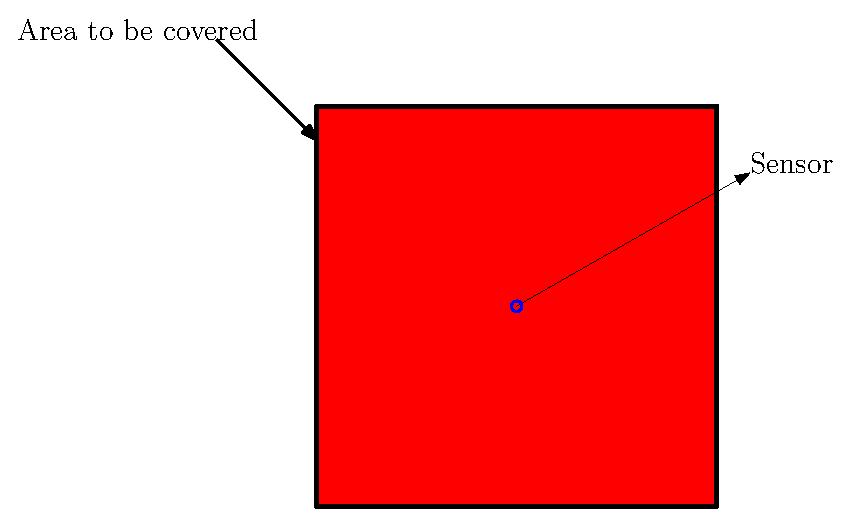
\includegraphics[scale=0.6]{motivation/coverage.eps}
\end{figure}
In red - the sensing coverage.
\end{frame}
%%
\begin{frame}[label=motivation2]{What Is Sensor Coverage?}
Why would we like to do that?
\begin{itemize}
\item Surveillance
\item Photographing
\item iRobot!
\end{itemize}

Those are all sensing coverage problem$^{1,2,3}$.

\footnotetext[1]{\tiny Nigam, N., Bieniawski, S., Kroo, I., \& Vian, J. (2012). Control of multiple UAVs for persistent surveillance: Algorithm and flight test results. IEEE Transactions on Control Systems Technology, 20(5), 1236–1251.}
\footnotetext[2]{\tiny Montijano, E., Sagues, C., \& Llorente, S. (2016). Multi-Robot Persistent Coverage with Optimal Times, (Cdc), 3511–3517.}
\footnotetext[3]{\tiny Loizou, S. G., \& Constantinou, C. C. (2016). Multi-Robot Coverage on Dendritic Topologies Under Communication Constraints, (Cdc).}
\end{frame}
%%
\begin{frame}[label=motivation3]{What Is Sensor Coverage?}
Coverage "Radius" - how much a sensor can sense

\begin{figure}[b]
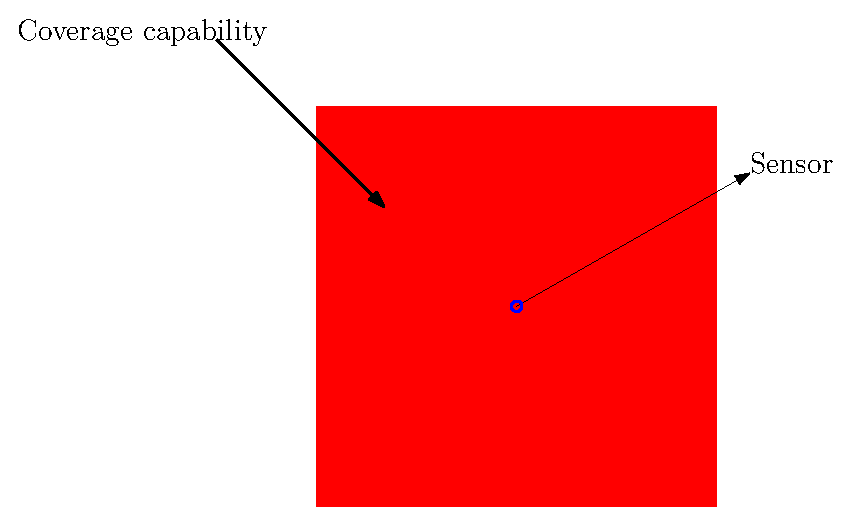
\includegraphics[scale=0.5]{motivation/coverage-radius.eps}
\end{figure}

In red - the sensor coverage \emph{radius}
\end{frame}
%%
\begin{frame}[label=motivation4]{Partial Coverage}
Single sensor - double the area size

\begin{figure}[b]
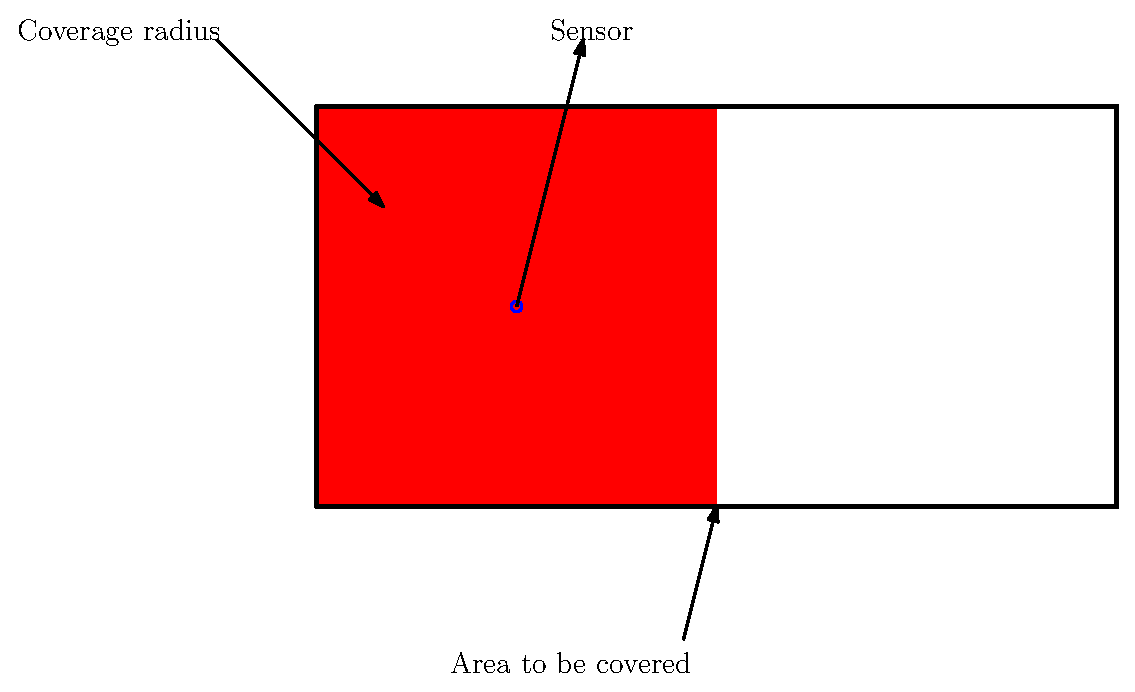
\includegraphics[scale=0.5]{motivation/partial-coverage.eps}
\end{figure}
In red - the sensor coverage. No \emph{full coverage}!
\end{frame}
%%
\begin{frame}[label=motivation5]{Full Coverage (again)}
Let's add another sensor!

\begin{figure}[b]
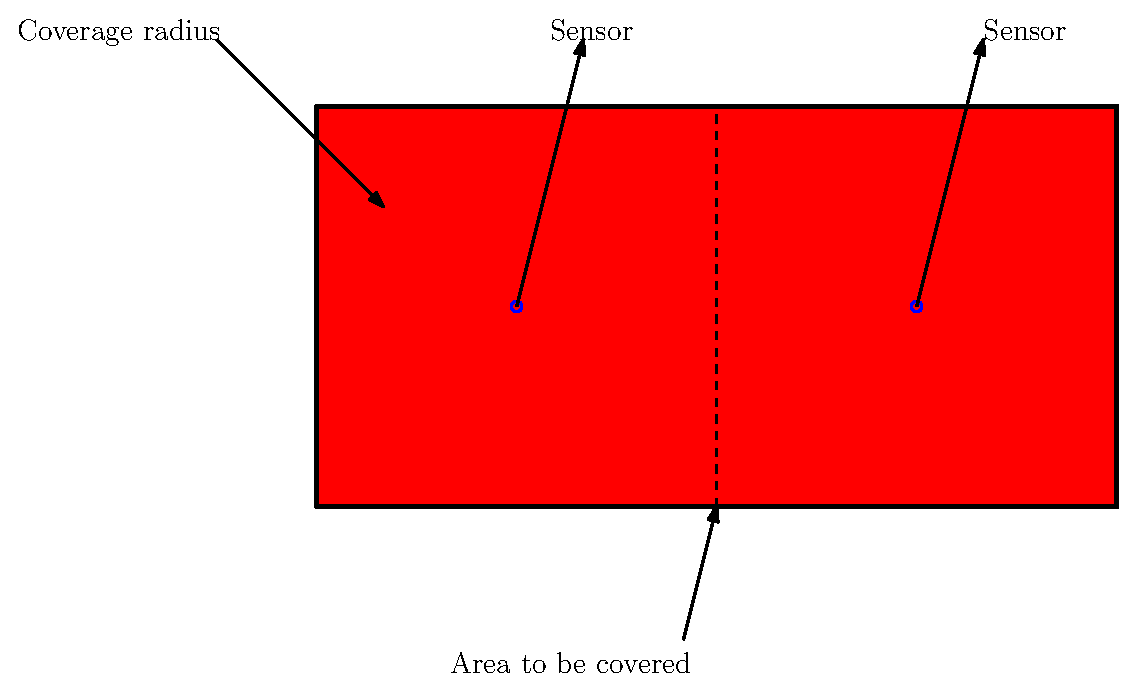
\includegraphics[scale=0.5]{motivation/partial-coverage-to-full.eps}
\end{figure}
New sensor added - now we have \emph{full coverage} once again!
\end{frame}
%%
\begin{frame}[label=motivation6]{Deployment}
Now we're dealing with multiple sensors. How should we configure them?

\begin{figure}[b]
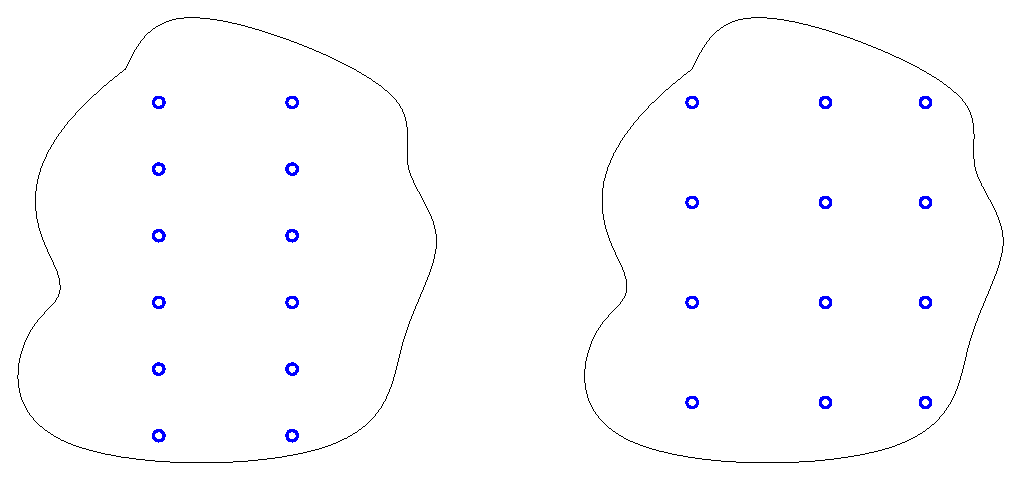
\includegraphics[scale=0.5]{motivation/deployment-configuration.eps}
\end{figure}
We have 12 sensors which we can \emph{deploy} in various configurations.
\end{frame}
%%
\begin{frame}[label=motivation7]{Deployment and full coverage}
Is it that simple?

\begin{figure}[b]
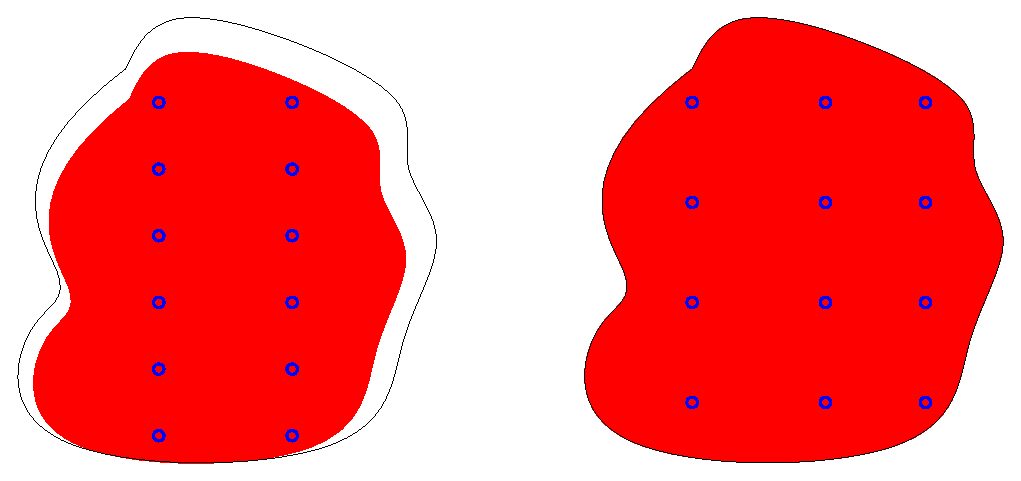
\includegraphics[scale=0.5]{motivation/deployment-configuration-partial-full-example.eps}
\end{figure}
One configuration results with full coverage, while the other one doesn't.
\end{frame}
%%
\begin{frame}[label=motivation8]{Deployment and full coverage}
Is it that simple?

\begin{figure}[b]
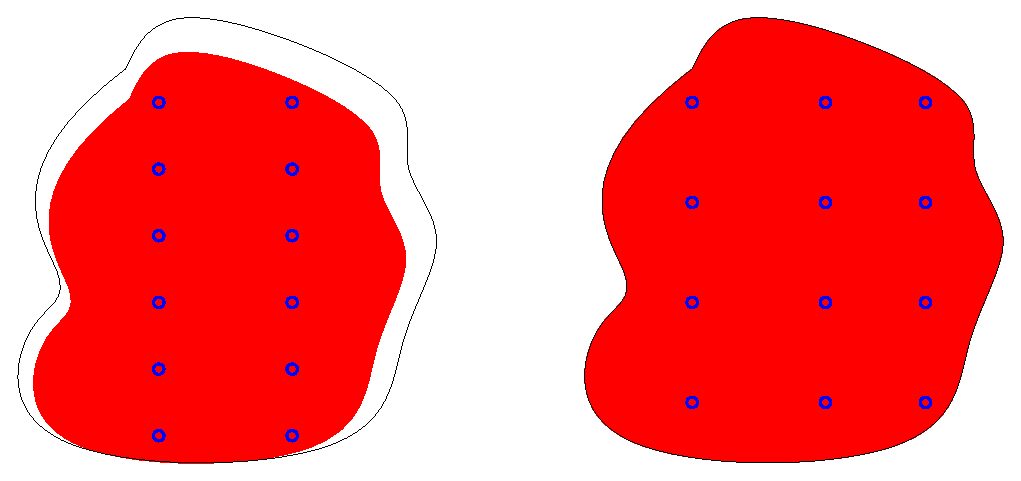
\includegraphics[scale=0.5]{motivation/deployment-configuration-partial-full-example.eps}
\end{figure}
One configuration results with full coverage, while the other one doesn't.
\end{frame}
%%
\begin{frame}[label=motivation9]{Partial Coverage}
There exists a deployment with 12 sensors which can cover the area. What if we only have 6 sensors?

\begin{figure}[b]
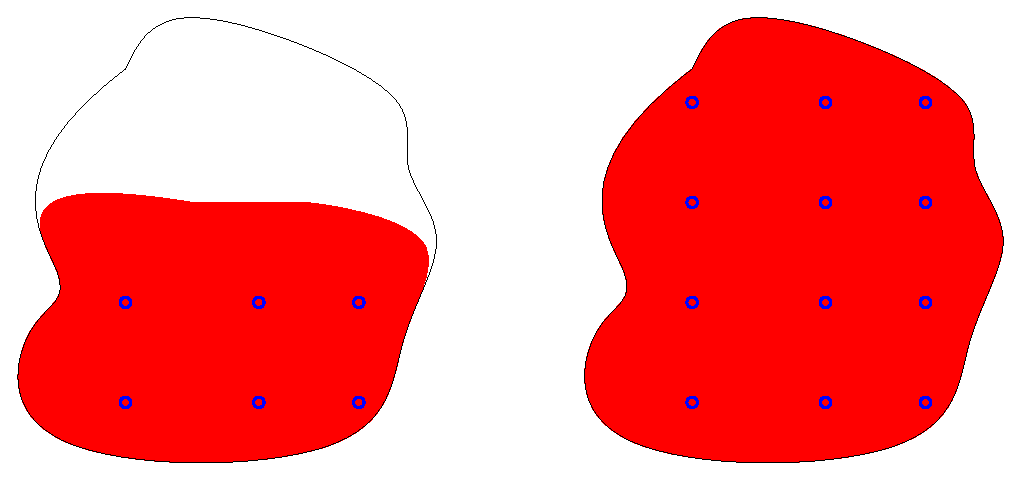
\includegraphics[scale=0.5]{motivation/deployment-configuration-partial-no-enough-sensors.eps}
\end{figure}
There doesn't exists a configuration that can supply full coverage!
\end{frame}
%%
\begin{frame}[label=motivation10]{Making it a bit more interesting...}
Let's say that we want to maintain coverage on a specific area, due to:
\begin{itemize}
\item Connection to home base
\item Maintain surveillance on a target
\item \ldots
\begin{figure}[b]
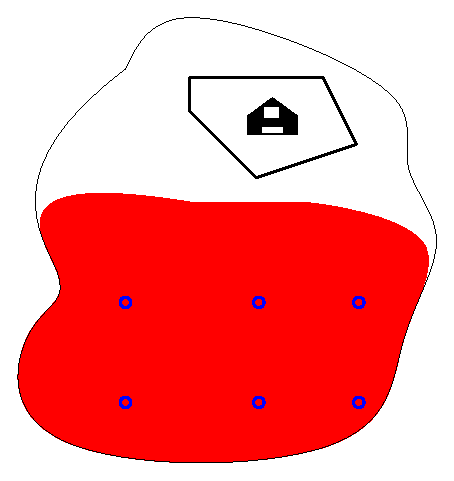
\includegraphics[scale=0.4]{motivation/deployment-configuration-coverage-constraint.eps}
\end{figure}
We have to take this into account when we build our coverage \emph{strategy}.
\end{itemize}
\end{frame}
%%
\begin{frame}[label=motivation11]{Partial Coverage Strategy}
Dealing with partial coverage - many possible behaviours:
\begin{itemize}
\item Set of trajectories $^{1,2,3}$
\item \emph{Tiling the area}
\item \ldots
\end{itemize}

By choosing any strategy, a \emph{coverage controller}$^4$ must be provided.

\footnotetext[1]{\tiny Atinç, G. M., Stipanović, D. M., Voulgaris, P. G., \& Karkoub, M. (2013). Supervised coverage control with guaranteed collision avoidance and proximity maintenance. Proceedings of the IEEE Conference on Decision and Control, 3463–3468.}
\footnotetext[2]{\tiny Hussein, I. I., \& Stipanovic, D. M. (2007). Effective Coverage Control for Mobile Sensor Networks With Guaranteed Collision Avoidance. IEEE Transactions on Control Systems Technology, 15(4), 642–657.}
\footnotetext[3]{\tiny Du, Q., Faber, V., \& Gunzburger, M., “Centroidal Voronoi Tessellations: Applications
and Algorithms,” SIAM Review, Vol. 41, No. 4, 1999, pp. 637–676.}
\footnotetext[4]{\tiny Cassandras, C. G., \& Li, W. (2005). Sensor Networks and Cooperative Control. Decision and Control, 2005 and 2005 European Control Conference. CDC-ECC ’05. 44th IEEE Conference On, 4237–4238.}
\end{frame}
%%
\begin{frame}[label=motivation12]{Partitioning as a strategy}
\emph{Partitioning} (or tiling) an area - cover a small part of the area each time.
\begin{itemize}
\item Main benefit - provide coverage of a subset of an area constantly.
\end{itemize}

Cortes et al.$^1$ provided a controller that know how to partition an area and provide coverage.

\begin{figure}[b]
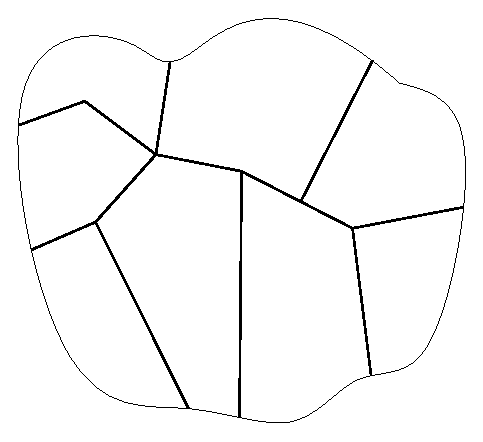
\includegraphics[scale=0.4]{motivation/partitioning.eps}
\end{figure}

\footnotetext[1]{\tiny Cortes, J., \& Martinez, S. (2004). Coverage control for mobile sensing networks.  IEEE Transactions on Robotics and Automation, 20(2), 243-255.}

\end{frame}

%%% Problem Formulation %%%
\subsection[Problem Formulation]{}
\begin{frame}[label=probformulation1]{Problem Formulation}
\begin{itemize}
\item There is some area $A \in \rR^{2}$ That we aim to cover.
\item A sub-area $A_{m} \subset A$ must be covered always (e.g. ground station).
\item There exist a set of \textbf{mobile} sensors $S = \left\{s_1 \ldots s_n\right\}$ located in positions $p_i(t) \in \mathbb{R}^2$ (for $i=1,\ldots,n$) at time $t$.
\begin{itemize}
\item The sensors can be controller with integrator dynamics $\dot{p_i}(t) = u$.
\item Each sensor can cover an area defined as $Cover\left( p_i, t \right)$.
\end{itemize}
\end{itemize}
\end{frame}
%%
\begin{frame}[label=probformulation2]{Problem Formulation}
\begin{itemize}
\item A configuration $c$ at time $t$ is the stack of the sensor positions at time $t$,
\begin{equation*}
c\left(t\right) = \bmat{
p_{1}^{T}\left(t\right)&\cdots&p_{n}^{T}\left(t\right)}^{T}\in\mathbb{R}^{2n}
\end{equation*}
\begin{itemize}
\item The coverage of a configuration $D\left( c\left( t \right) \right) = \cap Cover\left( p_i, t \right)$.
\end{itemize}
\end{itemize}
\begin{block}{Assumption}
$D\left( c\left( t \right) \right) \subset A$ - a single configuration \emph{can't} provide full coverage!
\end{block}
\end{frame}
%%
\begin{frame}[label=probformulation2]{Problem Formulation}
\begin{itemize}
\item A partition $j$ of the area $A$ is $pr_{j} \subset A$
\item The partitioning of $A, PR\left( A \right)$, built from $n$ partitions:
\begin{equation*}
PR\left( A \right) = \{ pr_{j} \mid \forall i \neq j,\textbf{ } pr_{i}\cap pr_{j} = \emptyset \textbf{ and }\cup pr_{j} = A \}
\end{equation*}
\end{itemize}
\end{frame}
%%
\begin{frame}[label=probformulation2]{Problem Formulation}
\begin{problem} \label{GeneralProblem}
\begin{enumerate}
\item Find partitioning such that for each partition $j, pr_{j} \cap A_m \neq \emptyset$ 
\item Find a deployment such that for each partition $j,$ and some given time $t, A_{pr_{j}} \subseteq D\left( c\left( t \right) \right)$
\end{enumerate}
\end{problem}
\end{frame}

%%%%%%%%%%%%%%%%%%%%%%%%%%%%%%%%%%%%%%%%%%
%%%%%%%%%%%%% MATH BACKGROUND %%%%%%%%%%%%
%%%%%%%%%%%%%%%%%%%%%%%%%%%%%%%%%%%%%%%%%%

\section[Mathematical Background]{Mathematical Background}
%%% Voronoi Partitioning %%%

\subsection[Voronoi Partitioning]{}
\begin{frame}[label=vorpart1]{Voronoi Partitioning}
\begin{center}
A little story about a town, a city planner and post offices...
\end{center}
\end{frame}
%%
\begin{frame}[label=vorpart2]{Voronoi Partitioning}
The Voronoi Diagram of a region $\Omega \subset \rsqr$ is the set of partitions $\mathcal{V} = \left\{V_{i} \mid \cup V_{i} = \Omega\right\}$, generated by the generators $\mathcal{Z} = \{z_1,\ldots,z_n\mid z_{i} \in \Omega\}$, such that
\begin{equation*} \label{Voronoi Definition}
V_{i} = \{q\in\Omega \mid \lVert q - z_i \rVert \leq \lVert q - z_j \rVert \forall z_i,z_j\in\mathcal{Z}\},
\end{equation*}
where $V_{i}$ corresponds to the $i$-th element of $\mathcal{Z}$, and $\lVert \cdot \rVert$ denotes the Euclidean distance.
\end{frame}
%%
\begin{frame}[label=vorpart3]{Voronoi Partitioning}
A rough example:
\begin{center}
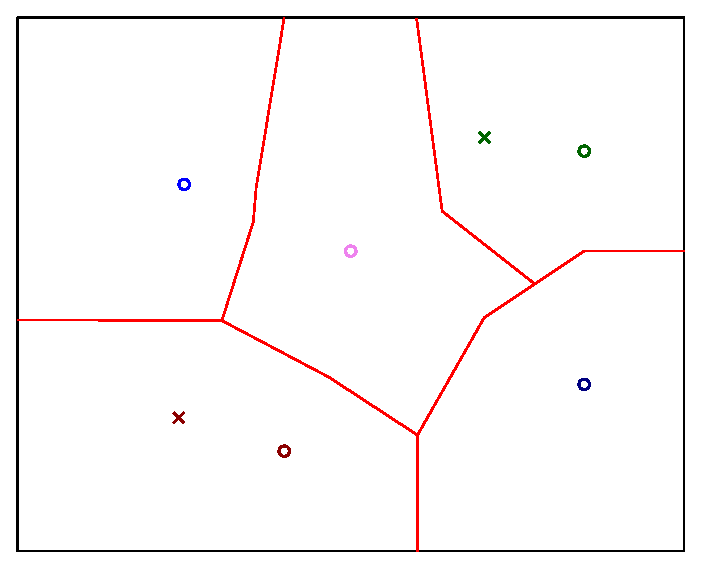
\includegraphics[scale=0.6]{background/Voronoi-example.eps}
\end{center}
Circles - generators, crosses - some point inside the appropriate partition.
\end{frame}
%%
\begin{frame}[label=centvorpart1]{Central Voronoi Tessellations}
\begin{center}
Let's get back to our city planner.
%\includegraphics[scale=0.5]{central-Voronoi-example.png}
\end{center}
\end{frame}
%%
\begin{frame}[label=centvorpart2]{Central Voronoi Tessellations}
Let us define a density function, $\rho_i$, for each Voronoi partition $V_{i}$. Then, we can define the center of mass for each partition as
\begin{equation*}
z_{i}^{*} = \frac{\int_{V_{i}}y\rho(y)dy}{\int_{V_{i}}\rho(y)dy}.
\end{equation*}
If a generator $z_{i} = z_{i}^{*} \, \forall \,V_{i}$, we call this partitioning a \emph{centroidal Voronoi tessellation} (CVT).
%%
Common examples for density function:
\begin{itemize}
\item $\rho(y) = \mathcal{N}\left( \mu, \sigma ^2 \right)$ (Gaussian distribution)
\item $\rho(y) = 1$
\end{itemize}
\end{frame}
%%
\begin{frame}[label=centvorpart3]{Central Voronoi Tessellations}
How it looks like?
\begin{center}
\includegraphics[scale=0.5]{background/central-Voronoi-example.png}
\end{center}
\end{frame}
%%
\begin{frame}[label=lloydsalg1]{Lloyd's Algorithm}
How do we calculate CVT?
\begin{algorithm}[H]
\caption{Lloyd's Algorithm} \label{LloydAlgo}
\begin{algorithmic}[1]
\State Calculate the Voronoi diagram for the current agents positions.
\State Calculate the center of mass for every cell.
\State Move the agents to the center of mass.
\State Repeat until convergence.
\end{algorithmic}
\end{algorithm}
\end{frame}
%%
\begin{frame}[label=lloydsalg2]{Lloyd's Algorithm}
So how do we calculate it?\\
Step 1:
\begin{figure}
\centering
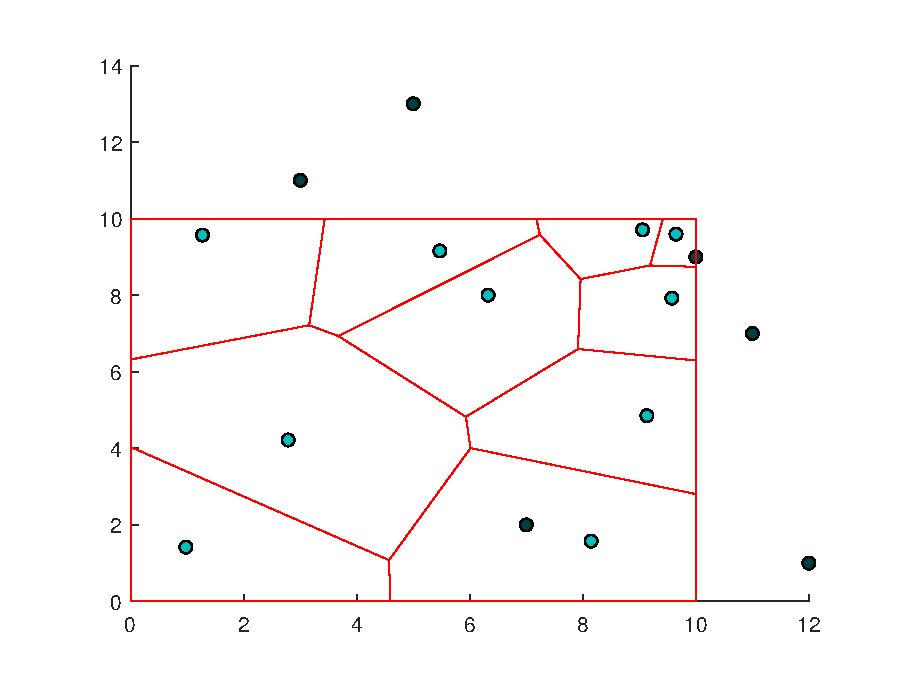
\includegraphics[scale=0.4]{background/cvt-calc-step1.eps}
\end{figure}
Black - initial guess, turquoise - after first iteration
\end{frame}
%%
\begin{frame}[label=lloydsalg3]{Lloyd's Algorithm}
Step 2:
\begin{figure}
\centering
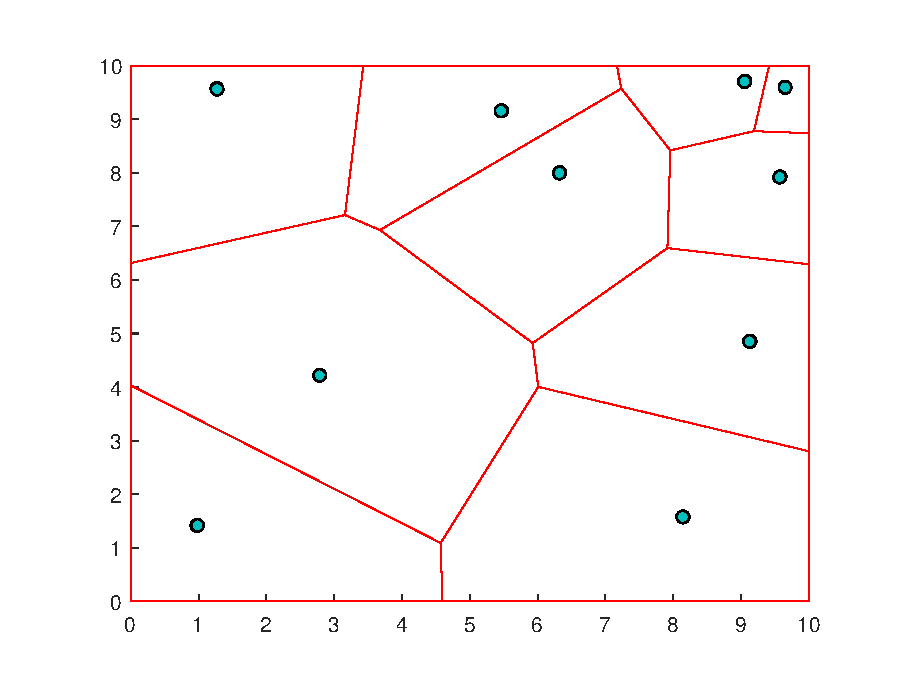
\includegraphics[scale=0.4]{background/cvt-calc-step2.eps}
\end{figure}
Black - first iteration solution, turquoise - after second iteration
\end{frame}
%%
\begin{frame}[label=lloydsalg4]{Lloyd's Algorithm}
Step 2 - zoom in:
\begin{figure}
\centering
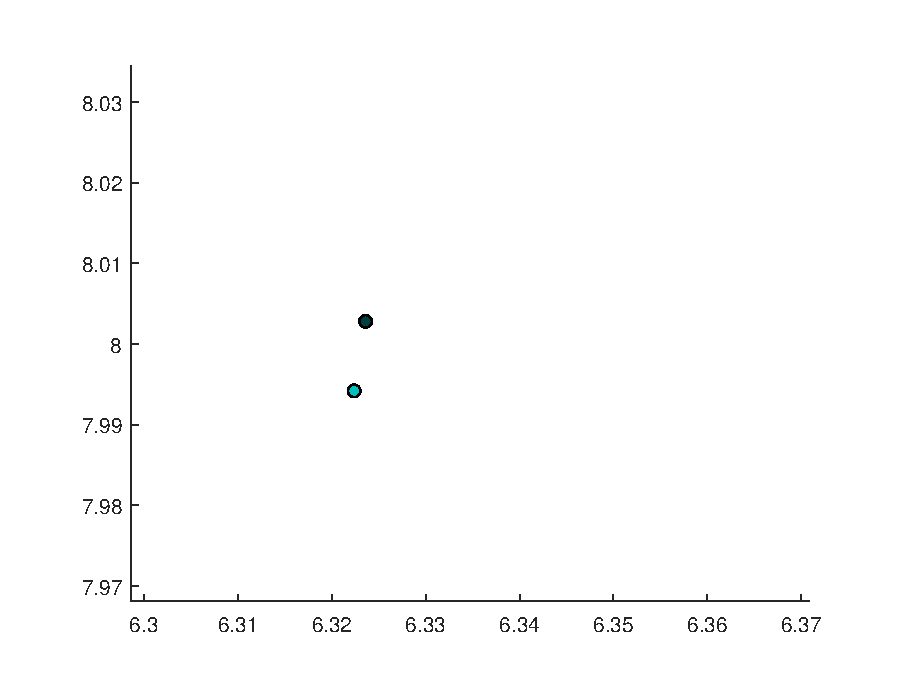
\includegraphics[scale=0.4]{background/cvt-calc-step2-zoom.eps}
\end{figure}
Almost converged...
\end{frame}
%%
\begin{frame}[label=lloydsalg5]{Lloyd's Algorithm}
After n iterations:
\begin{figure}
\centering
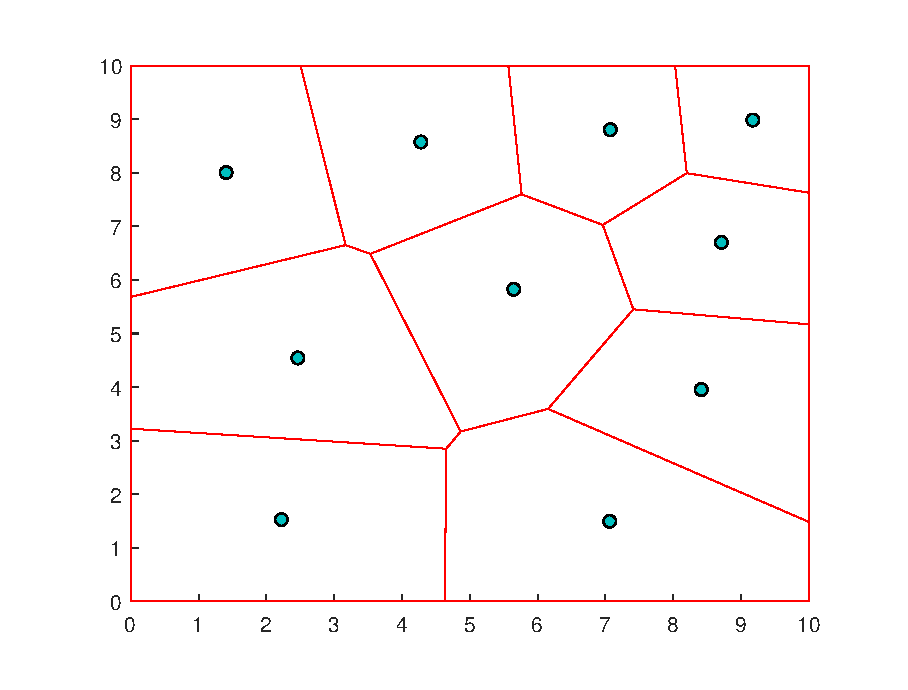
\includegraphics[scale=0.4]{background/cvt-calc-stepn.eps}
\end{figure}
\end{frame}
%%
\begin{frame}[label=lloydsalg6]{Lloyd's Algorithm}
[Cortes2004] proposed a continuous time controller for Lloyd's algorithm. If we define agent $i$ position as $p_i$ and the $i$'s partition centroid as $C_{V_{i}}$, then for some proportional constant $k_{p}$, the controller can be defined as:
\begin{equation*} \label{Lloyds contoller}
u_{i} = -k_{p}\left( p_i - C_{V_{i}} \right)
\end{equation*}

\begin{figure}[b]
\centering
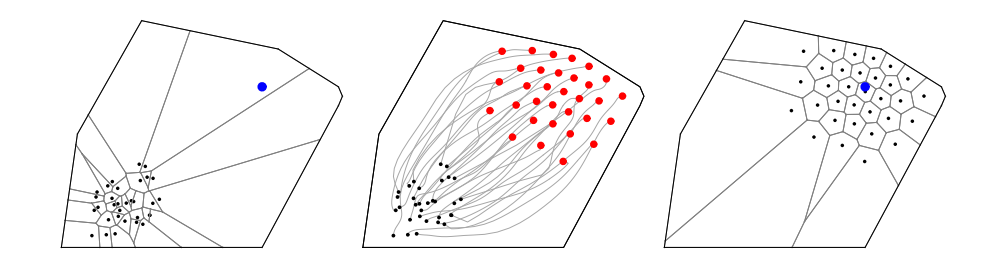
\includegraphics[scale=0.3]{Lloyds-alg-from-cortes.png}
\caption{A simulation from [Cortes2004] with 32 agents and Gaussian density function}
\end{figure}
\end{frame}
%%
\begin{frame}[label=lloydsalg7]{Lloyd's Algorithm}
Another important result in [Cortes2004] is that this controller is locally asymptotically stable. Proof is given in the paper using the direct Lypunov methos, using the following potential function:
\begin{equation*}
\mathcal{H_{V}}\left( P \right) = \sum_{i=1}^{n} J_{V_i,C_{V_i}} + \sum_{i=1}^{n} M_{V_i} \norm{p_i - C_{V_i}}^2
\end{equation*}
Where:
\begin{itemize}
\item P - the set of the agents positions
\item $V_i$ - the $i$'th Voronoi partition
\item $J_{V_i,C_{V_i}}$ - the polar moment of inertia of $V_i$ about its centroid $C_{V_i}$
\item $M_{V_i}$ - the $i$'th partition "mass"
\end{itemize}
\end{frame}
%%
\begin{frame}[label=lloydsalg8]{Lloyd's Algorithm}
An important thing we have to remember - Lloyd's algorithm is NOT a distributed calculation!
\end{frame}

%%%%%%%%%%%%%%%%%%%%%%%%%%%%%%%%%%%%%%%%%%
%%%%%%%%%%%%% PROBLEM SOLUTION %%%%%%%%%%%
%%%%%%%%%%%%%%%%%%%%%%%%%%%%%%%%%%%%%%%%%%

\section[Problem Solution]{Problem Solution}

\subsection[Projected Lloyd's Algorithm]{}
\begin{frame}[label=projlloydsalgo1]{Projected Lloyd's Algorithm}
We should supply a solution for the "Coverage Constraint" \pause
\begin{block}{Reminder}
A given area inside the area $A_{m} \subset A$ must be covered always
\end{block}\pause
We came up with a rather simple solution for this problem.
\end{frame}

\begin{frame}[label=projlloydsalgo2]{Projected Lloyd's Algorithm}
\begin{algorithm}[H]
\caption{Projected Lloyd's Algorithm (PLA)}\label{ProjLloydsAlgorithm}
\begin{algorithmic}[1]
\State Calculate the Voronoi diagram for the current agents positions.
\State Calculate the center of mass for every cell.
\State Project the center of mass of every cell to the area constraint limiting polygon.
\State Move the agents the projected center of mass.
\State Repeat until converge.
\end{algorithmic}
\end{algorithm}

Writing this algorithm as a controller:
\begin{equation} \label{ProjectedLloydsContol}
u_{i} = -k_{p}\left( p_i - \textit{proj}\left( C_{V_{i}} \right) \right)
\end{equation} 
\end{frame}

\begin{frame}[label=projlloydsalgo3]{Projected Lloyd's Algorithm}
In the following example:
\begin{itemize}
\item Left - regular CVT, build with the original Lloyd's Algorithm.
\item Right - A partitioning built with the PLA.
\end{itemize}
\begin{figure}
\centering
\begin{minipage}{.4\textwidth}
  \centering
  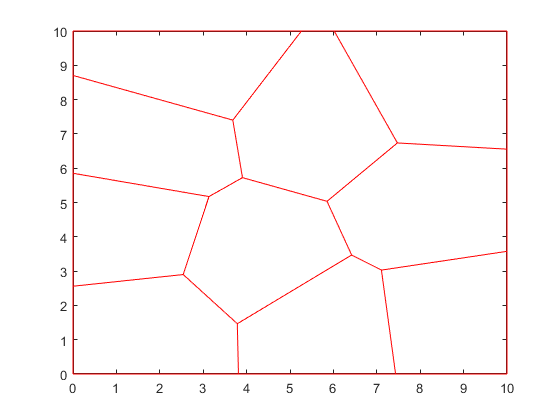
\includegraphics[scale=0.3]{proj-lloyds-off.png}
\end{minipage}
\begin{minipage}{.4\textwidth}
  \centering
  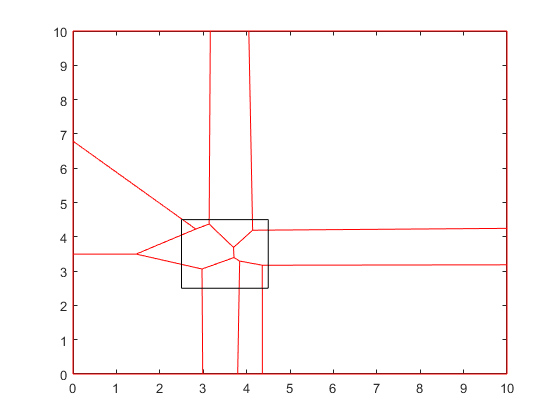
\includegraphics[scale=0.3]{proj-lloyds-on.png}
\end{minipage}
\end{figure}

\end{frame}

\begin{frame}[label=projlloydsalgotheorem]{Projected Lloyd's Algorithm}
\begin{theorem}
The projected Lloyd's Algorithm is locally asymptotically stable
\end{theorem}

As the projection is a linear operator, the controller is also locally asymptotically stable, and the proof is virtually the same as was given by Cortes et al. The proof is based on a proposal of Lyaponov function, and then using the direct Lyaponov method to prove the stability
\end{frame}

\begin{frame}[label=projlloydsalgoproof]{Proof of stability}
As the projection is a linear operator, the controller is also locally asymptotically stable, and the proof is virtually the same as was given by Cortes et al.\\

\end{frame}

\subsection[Problem Solution Algorithm]{}
\begin{frame}[label=probsolalg1]{Problem Solution Algorithm}
So far, we've given solution for:
\begin{itemize}
\item Covering a given area using Voronoi partitioning
\item Partition and area such that the coverage constraint is fulfilled.
\end{itemize}

Therefore, we are ready for the problem solution algorithm...
\end{frame}

\begin{frame}[label=probsolalg2]{Problem Solution Algorithm}
\begin{algorithm}[H]
\caption{Problem Solution Algorithm}\label{GeneralProbSolution}
\begin{algorithmic}[1]
\State Using some random initial guess, partition the whole area using PLA.
\State For each partition (assuming that the agents can actually cover each partition with their coverage radius), calculate the CVT. The initial positions for the CVT calculation is the previous partition CVT.
\end{algorithmic}
\end{algorithm}
\end{frame}

\subsection[Lloyd's Algorithm and Formation Control]{}
\begin{frame}[label=lloydsandformation1]{Lloyd's Algorithm and Formation Control}
\begin{itemize}
\item<1-> Problem solved.
\item<2-> Make it more interesting...
\item<3-> Combine Lloyd's Algorithm with distance-based formation control! \begin{itemize}
\item<4-> create and maintain spatial properties partially or fully (We do not provide a condition where this combination meets the requirements).
\end{itemize}
\end{itemize}
\end{frame}

\begin{frame}[label=lloydsandformation2]{Lloyd's Algorithm and Formation Control}
As both of the controllers are convex, we propose to simply combine them with some coefficient:\\
\begin{equation}
    u_{i} = \alpha \left(-k_{p}\left( p_i -C_{V_{i}} \right)\right) +
    \left( 1-\alpha \right)\left[-\sum_{i \sim j} \left( \norm{p_{i} - p_{j}}^{2} - d_{ij}^2 \right) \left( p_{i} - p_{j} \right)  \right] 
    \label{Combined Controller}
\end{equation}\pause
\begin{theorem}
The combined controller is Locally Asymptotically Stable
\end{theorem}
\end{frame}

\begin{frame}[label=lloydsandformation3]{Lloyd's Algorithm and Formation Control}
How to prove:
\begin{itemize}
\item Pretty long and technical, based on Lyapunov function.
\item We know the Lyapunov function of each controller - Let's combine!
\item After long calculations, we can show using the Lyapunov direct method that this controller is locally asymptotically stable.
\item In the same way, we can show it works with the PLA.
\end{itemize}
\end{frame}



%%%%%%%%%%%%%%%%%%%%%%%%%%%%%%%%%%%%%%%%%%
%%%%%%%%%%%%% Simulations %%%%%%%%%%%%%%%%
%%%%%%%%%%%%%%%%%%%%%%%%%%%%%%%%%%%%%%%%%%

\section[Simulations]{Simulations}
\subsection[Some Simulation]{}
\begin{frame}[label=sl3]{Some Simulation}
List of simulations to create:
\begin{itemize}
\item 3 agents, 5 big partitions, no formation, no PLA
\item 3 agents, 5 big partitions, no formation, PLA
\item 10 agents, 5 big partitions, no formation, PLA
\item 6 agents, 5 big partitions, some formation, PLA
\end{itemize}
\end{frame}

%%%%%%%%%%%%%%%%%%%%%%%%%%%%%%%%%%%%%%%%%%
%%%%%%%%%%%%%% Formation %%%%%%%%%%%%%%%%%
%%%%%%%%%%%%%%%%%%%%%%%%%%%%%%%%%%%%%%%%%%
\subsection[Distance-Based Formation Control]{}
\begin{frame}[label=distanceformation1]{Formation Control}
For a complete background, some prior knowledge on algebraic graph theory is needed. Let's simplify:
\begin{itemize}
\item We have agents $1 \ldots n$ on positions $p_{i}$ \pause
\item Goal - agents $i,j (i \neq j)$ will be at distance $d_{ij}$ \pause
\item Only $\varepsilon$ agents can share information.
\end{itemize}
\end{frame}

\begin{frame}[label=distanceformation2]{Formation Control}
\begin{figure}[t!]
\centering
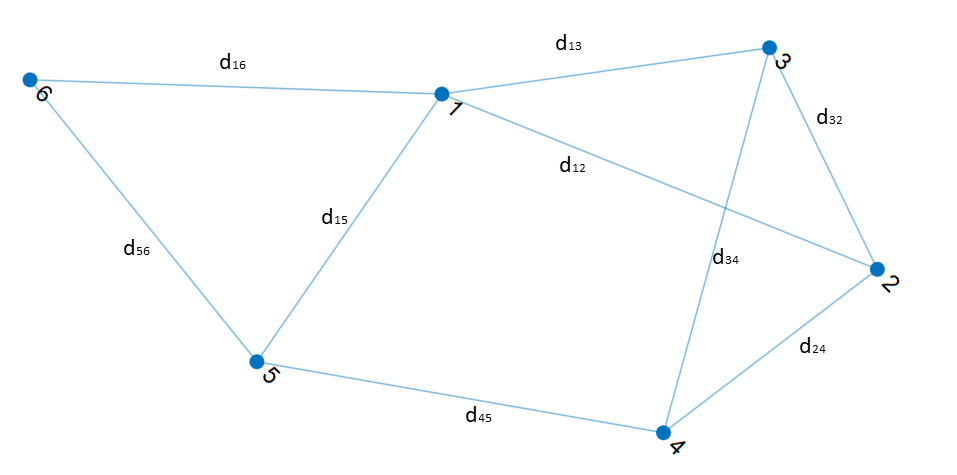
\includegraphics[scale=0.42]{graph-example.png}
\end{figure}
\end{frame}

\begin{frame}[label=distanceformation3]{Formation Control}
For a single agent $p_i$, the controller will have the following form:
\begin{equation}
    \dot{p_{i}} = -\sum_{i \sim j} \left( \norm{p_{i} - p_{j}}^{2} - d_{ij}^2 \right) \left( p_{i} - p_{j} \right)
    \label{formation controller}
\end{equation}
This controller is locally asymptotically stable.
\end{frame}

\subsection[Projection Operator]{}
\begin{frame}[label=projoperator]{Projection Operator}

The projection linear operator is defined as a linear transformation $P$ from a vector space to itself such as $P^2 = P$. In other words, the transformation $P$ is idempotent.

\end{frame}
\end{document}
